% !TEX root = ../main.tex

\section{Implementation} \label{sec:implementation}

The application is written in Java. Given that Java is an object-oriented
language, the implementation and design choices reflect this. 

\subsection{Genetic algorithm Implementation}

The smallest component in a genetic algorithm is the allele. For the final implementation, the
allele class contains two fields: \texttt{index} representing the index of a
break point and \texttt{methodBreakPoint} being of an abstract object
\texttt{BreakPoint}. A break point is decided by the fitness method and thus
this field needs to be rather flexible. This in turn means that each fitness
method needs its own. More on fitness methods in
section~\ref{sec:fitness-methods}. 

The alleles is stored in the genome. The genome class has one field which is an
\texttt{ArrayList} of alleles. Each index in the genome is instead called a
\textit{gene} to fit the narrative. Ie. there is an allele at a gene in the
genome. 

The genome makes sure the alleles are always in ascending order, sorting the break
point indexes. This makes calculating fitness and displaying the break points
much easier. 

An individual consists of a genome, a fitness value and list of \textit{fitness nodes}.
More on the fitness nodes in section~\ref{sec:fitness-methods}. The fitness
value is a measure of how well the individual matches with a given time series.
This could cause trouble if the same individual is mathed against multiple time
series. This is never the case and will never be a problem. 

The individual always has two breakpoints with indexes $0$ and $T$ respectively.
The individual also has functionality like adding and removing break points. The
individual can also tell if it has an allele with a certain break point index.
Here, the method \texttt{geneOf} from the genome class is used. This method
loops through all alleles in the genome and returns the gene containing the first allele matching a
condition. The condition itself is specified through a \texttt{Predicate}
allowing for lambda notation. 
\begin{lstlisting}
public boolean breakPointAtIndex(int breakPointIndex) {
    // geneOf returns > 0 if an allele a has the break point index
    return genome.geneOf(a -> a.getIndex() == breakPointIndex) != -1;
}
\end{lstlisting}
where \texttt{a} means an allele. 

All the individuals are stored in a population. A population is a simple array
of individuals. It is able to retrieve the fittest individual and replacing the
least fit individual with a new individual. At one point, the population class
stored the individuals in a \textit{priority queue}. Although faster for
replacing the least fit individual, the code itself became more convoluted.
Since the population can contain at most 100 individuals, the gain in speed did
not seem that important. 

The population class is also responsible for initializing itself with a number
of random individuals as in the pseudo code. Here, it also assigns the fitness
to the individuals. 

See figure~\ref{fig:class-diagram-ga} for a class diagram of the elements in the
genetic algorithm part/package. 

\begin{figure}[ht]
    \centering
    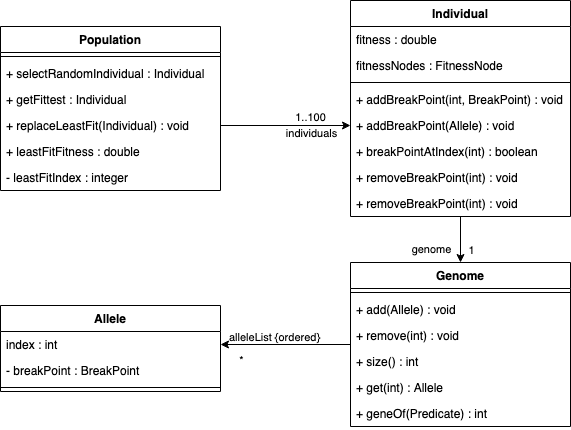
\includegraphics[width=.8\textwidth]{fig/class-diagram-ga.png}
    \caption{Class diagram for the genetic algorithm elements}
    \label{fig:class-diagram-ga}
\end{figure}


\subsection{Fitness methods} \label{sec:fitness-methods}

For this project, only the rectangle fitness method has actually been
implemented. But the rectangle fitness class is based on an abstract fitness
class. This means that new fitness methods can easily be implemented as
sub-classes of the abstract class. All fitness classes must have the following
following: 
\begin{description}
    \item[fitnessOf] A method for calculating the fitness of an individual given
    a time series. 
    \item[newBreakPoint] Each fitness method has its own kind of break point
    containing some information. This is an object of the \texttt{BreakPoint}
    object and must also be unique for each model. 
    \item[getModelCode] The model code is simply a string for the name when
    choosing the fitness in the GUI. 
    \item[getNodes] When drawing the fitness in the GUI, each fitness method
    must have its own way of displaying break points. For rectangles, this is
    drawing rectangles on the graph, see section~\ref{sec:graph-implementation}.
    A \texttt{FitnessNode} is an (abstract) object which stores some information
    relevant for drawing on the graph. Each fitness method must have its own
    kind of \texttt{FitnessNode}. 
\end{description}


\subsection{Loading the time series and range trees}

The time series data files are stored in the \textit{JSON} format. To load
these, Googles Maven package \textit{JSON.simple} is used. That package has a
great \texttt{get}-method to retrieve information under a given string name, ie.
\texttt{get("observations")} or \texttt{get("time")}. 

For this project, when reading a data file with more than 1 dimension, an
exception is thrown. For all data files with 1 dimension, the files are read
easily as JSON.simple handles the files very much like arrays. 

When all the data is loaded, the observation values are read into a range tree.
This is a custom data structure implemented in Java. The range tree is
implemented as mentioned in section~\ref{sec:range-tree-design}. The code for
building the tree and making queries can be found in
appendix~\ref{app:code-snippets}. 

In the implementations above, a \texttt{MinMax} object is used. This is a simple
object to store a minimum and a maximum value. 

\subsection{The structural breaks algorithm}

The algorithm for finding structural breaks is found in the class
\texttt{BreakPointAlgorithm}. This is the brain of the system and the
\textit{model} in model-view-controller. This class itself manipulates the other
objects in a manner much like the handed out pseudo code. Thus, the
implementation here is not very interesting. A class diagram of the break point
algorithm together with time series and fitness models is shown in figure
~\ref{fig:class-diagram-algorithm} in appendix~\ref{app:class-diagrams}.


\subsection{GUI: Displaying the graph and break points}
\label{sec:graph-implementation}

The GUI itself is made in the FXML language from JavaFX with the help of the
application \textit{SceneBuilder}. Styling has been done in CSS. Given the simplicity of the application, only one
scene has been designed as is ever in use. This has made 
designing the GUI a breeze. 

Writing GUI in FXML makes the separation of \textit{view} and
\textit{controller} very apparent. The view is in the FXML language. The
controller is in Java. 

\begin{figure}[ht]
    \centering
    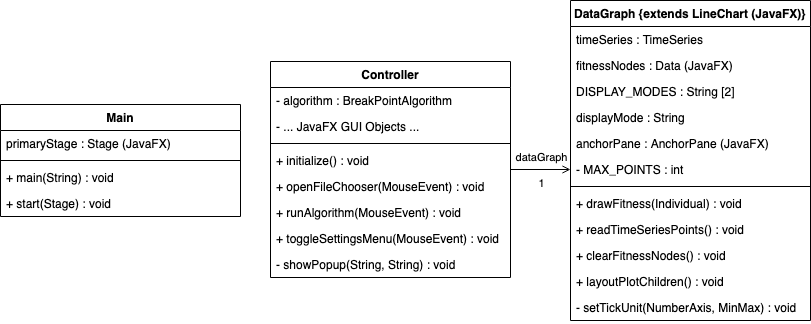
\includegraphics[width=.8\textwidth]{fig/class-diagram-controller.png}
    \caption{Class diagram for controller and main}
    \label{fig:class-diagram-controller}
\end{figure}

The controller handles all the interactions from the user. This is methods like
\texttt{openFileChooser} which opens the operating systems own file chooser to
select a JSON file. With the file chooser open, only JSON files can be chosen.
The controller then loads the time series sets that as the time series in the
\texttt{BreakPointAlgorithm} and displays the time series in the GUI. The
controller also tells the \texttt{BreakPointAlgorithm} to find the break points
when the relevant button is pressed. 

The controller also initializes all the slider and drop-down menus. For the
drop-down menus this means adding all the elements and adding a listener to get
the selection when a user selects an element. For the sliders, the initial value
is set as the same as the \texttt{BreakPointAlgorithm} using the static class
\texttt{InitValues}. Listeners are added to observe the changing values. For
most, this means updating the value display in the GUI and updating the relevant
value in \texttt{BreakPointAlgorithm}. For the probability values a bit more
work is needed: The math from section~\ref{sec:gui-design} is implemented also. 

\begin{figure}[ht]
    \centering
    \begin{subfigure}[b]{.48\textwidth}
        \centering
        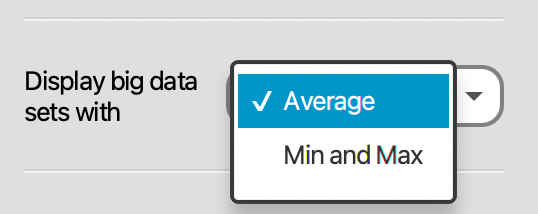
\includegraphics[width=\textwidth]{fig/drop-down-menu.png}
        \caption{Drop-down menu example. }
        \label{fig:gui-drop-down}
    \end{subfigure}
    \hfill
    \begin{subfigure}[b]{.48\textwidth}
        \centering
        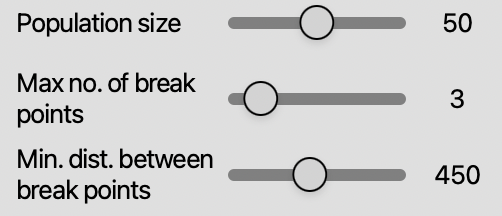
\includegraphics[width=\textwidth]{fig/sliders.png}
        \caption{Slider example.}
        \label{fig:gui-slider}
    \end{subfigure}
    \caption{Examples of initialized and working menus and sliders}
    \label{fig:gui-controls}
\end{figure}

The controller only makes one \textit{change} to the view: Replacing a
placeholder \texttt{LineChart} with a custom \texttt{LineChart} object
\texttt{DataGraph}. The reason to create a custom object is to draw the fitness
markers on the graph. JavaFX' \texttt{LineChart} is \textit{not} user-friendly
in this regard and it has to be done through the private
\texttt{layoutPlotChildren} method. Thus, a new object needed to be created. 

Getting the break point markers on the graph was yet another challenge. First,
the scaling from width and height on the time series to width and height on the
display on the screen needed to be calculated. Then, the node has to be placed
on the graph which, with the scale, was somewhat easy but took forever to get
right.  

At first, the markers was placed directly on the \texttt{LineChart} but it
was changed to be placed on a \texttt{AnchorPane}. The decision to move to
\texttt{AnchorPane} was motivated by one thing: The different type of
nodes/figures in JavaFX has different parameters to decide the positioning. In
an \texttt{AnchorPane}, the positions can be made to only $x$ and $y$. Thus, the
fitness nodes must have an $x$ and $y$ position for upper left corner, and they
must also have a width and height. For the fitness node itself, these values are
in the scope of the time series. The transformation is done in
\texttt{DataGraph} itself
and is only graphical. 

All this work payed off as the GUI is completely scalable and the fitness
markers follows the scaling of the window, see figure~\ref{fig:gui-scaling}

\begin{figure}[ht]
    \centering
    \begin{subfigure}[b]{.48\textwidth}
        \centering
        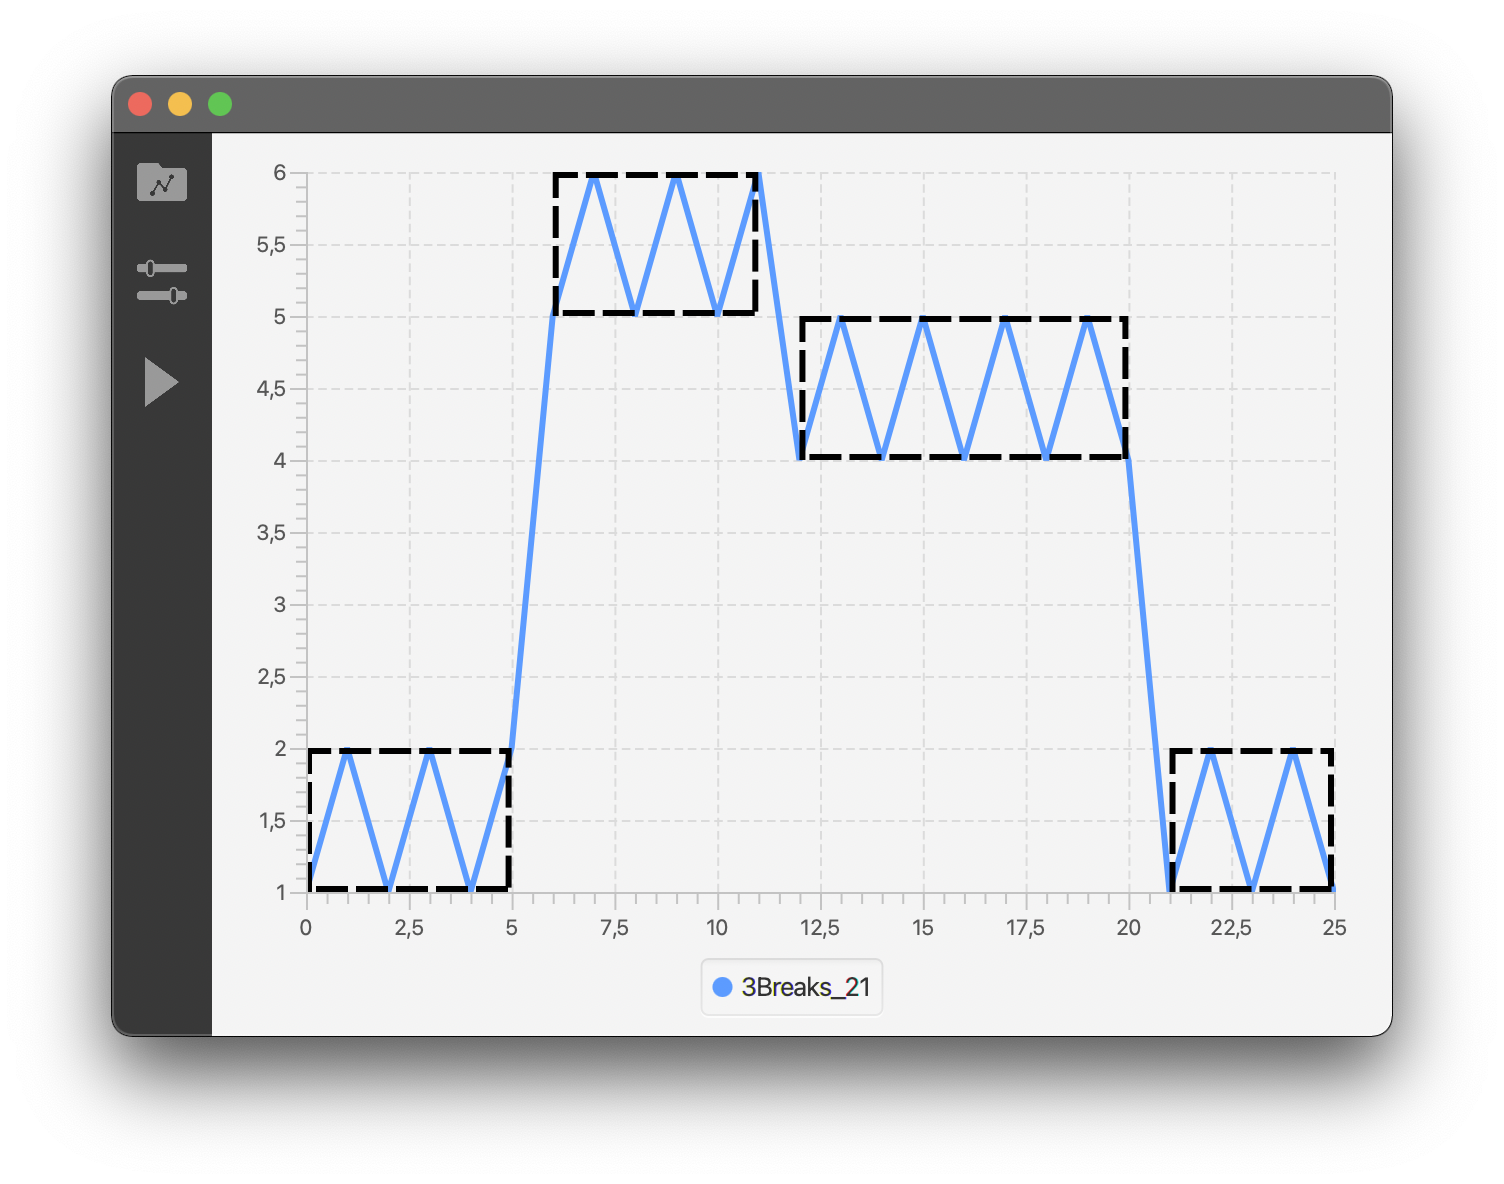
\includegraphics[width=\textwidth]{fig/gui-small-screen.png}
        \caption{GUI in 480 x 640 pixels}
        \label{fig:gui-small-screen}
    \end{subfigure}
    \hfill
    \begin{subfigure}[b]{.48\textwidth}
        \centering
        \raisebox{7mm}{
            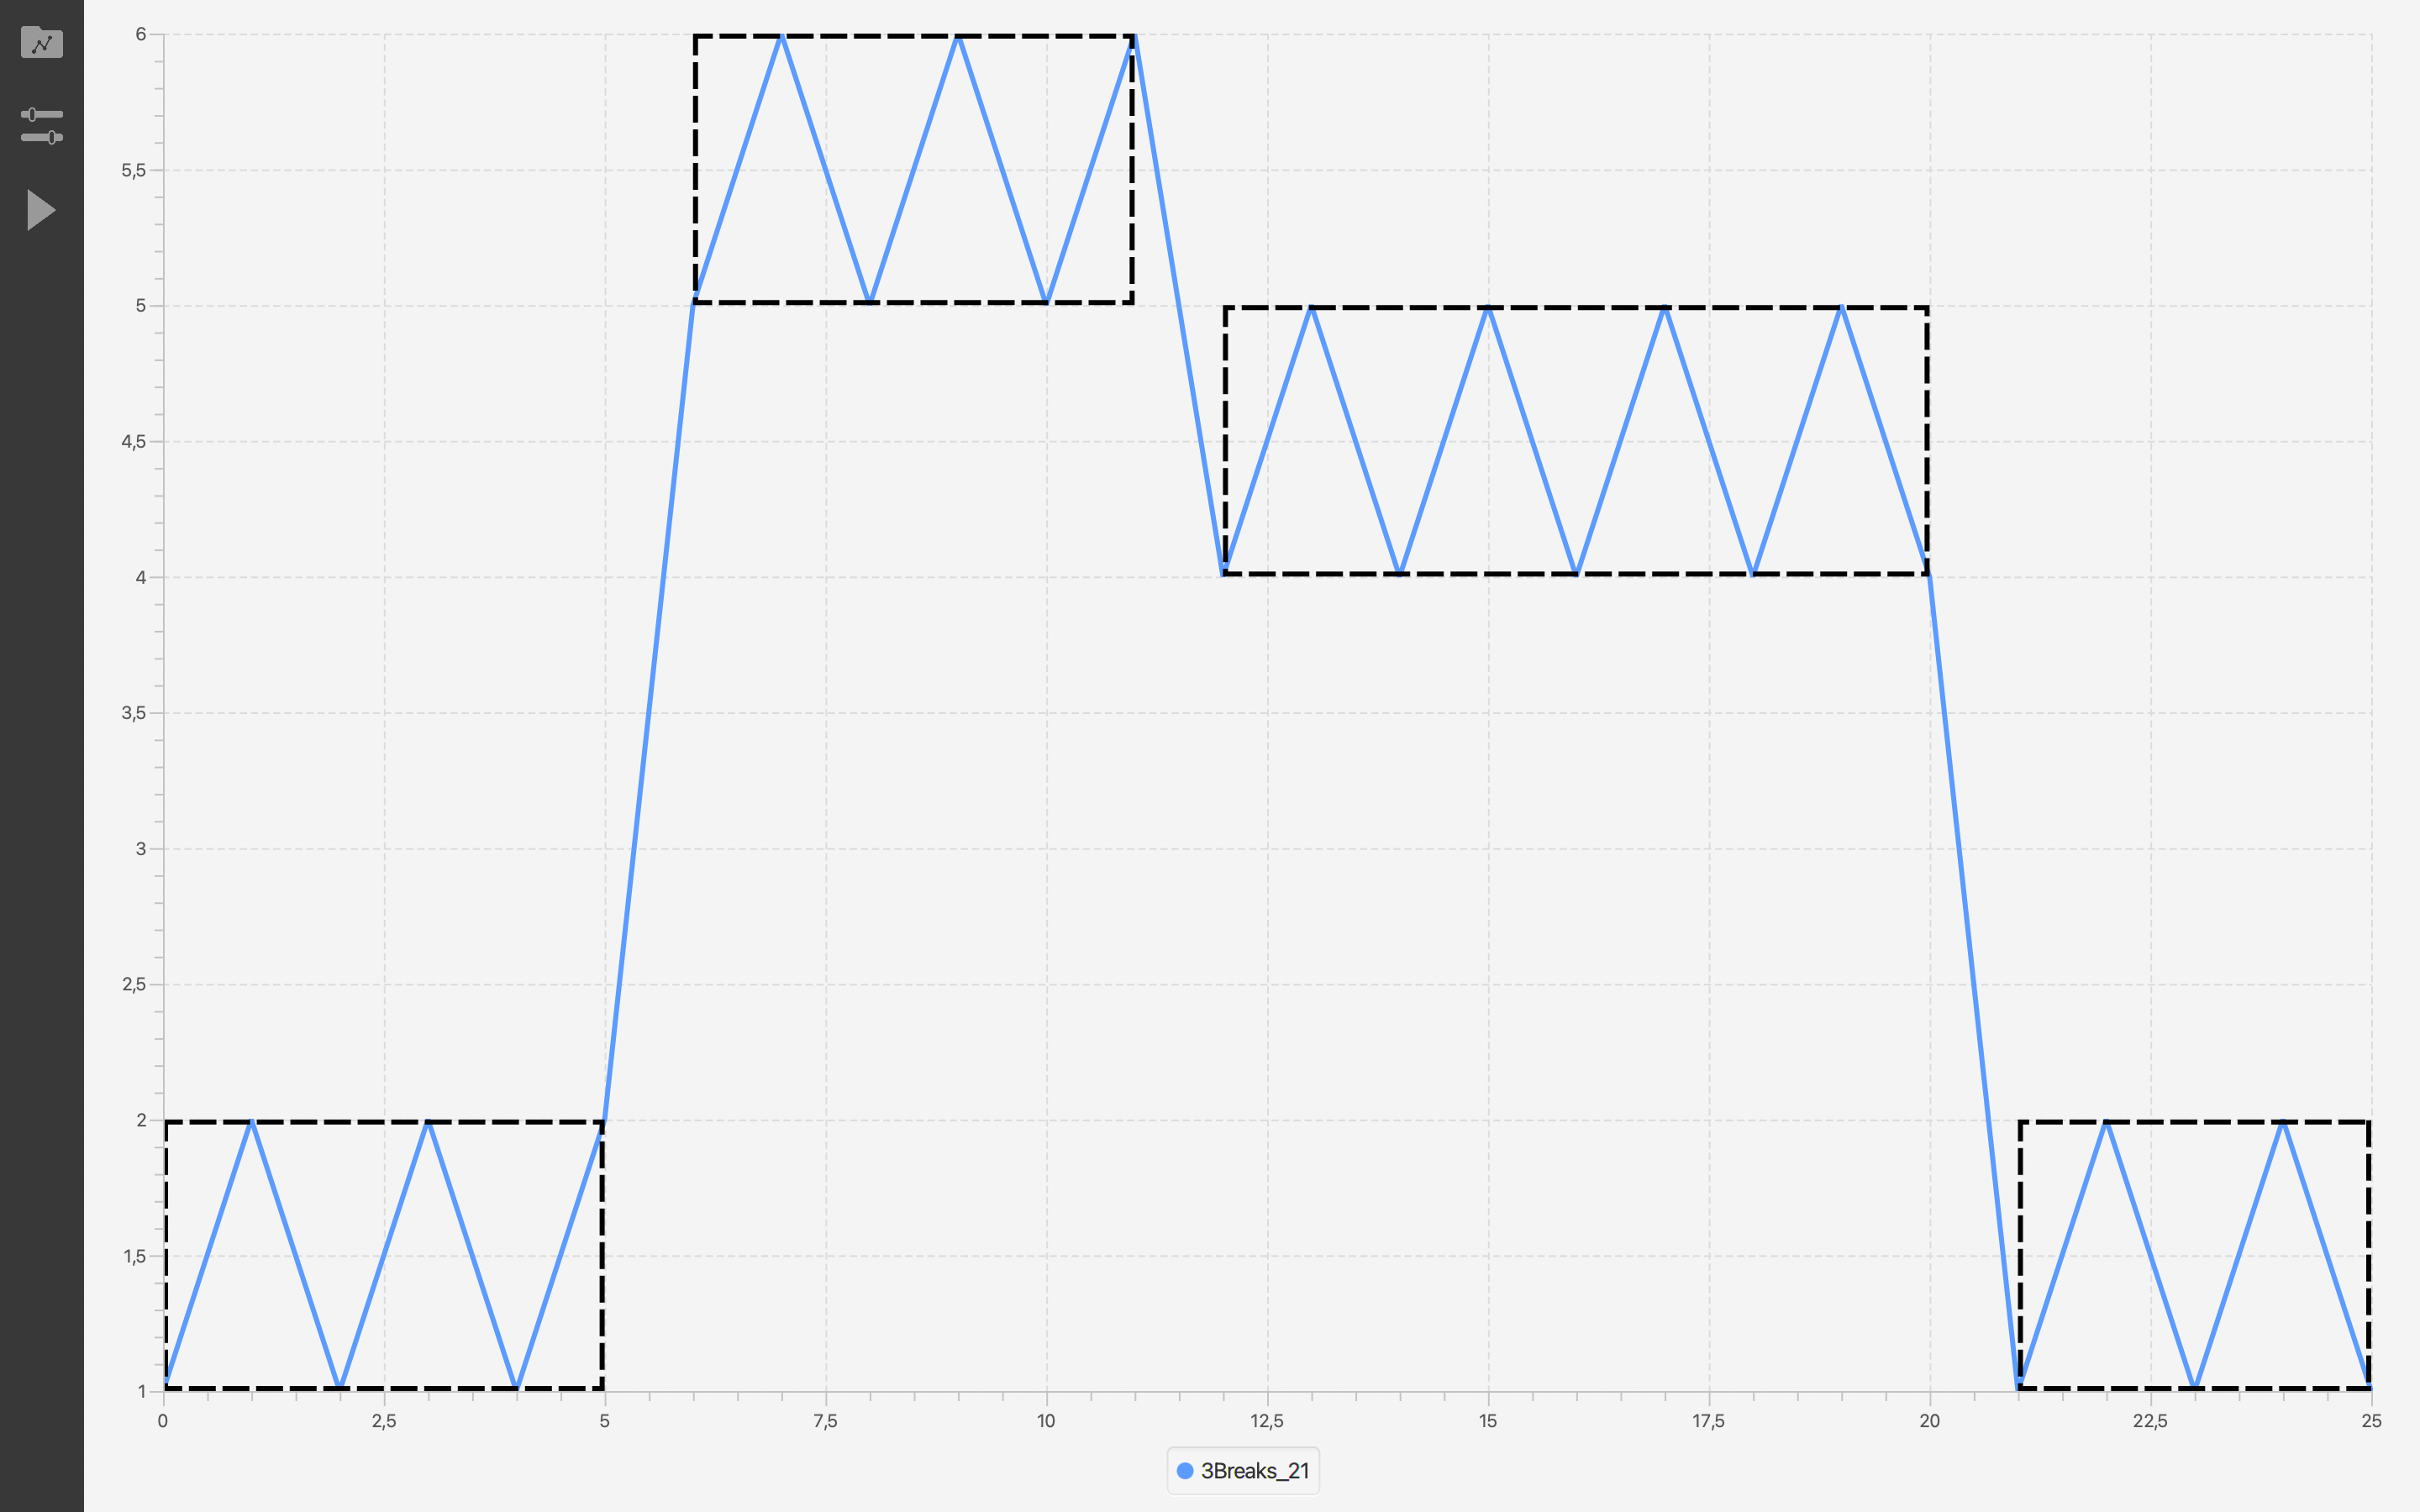
\includegraphics[width=\textwidth]{fig/gui-full-screen.png}
        }
        \caption{GUI in full screen, 2560 x 1600 pixels}
        \label{fig:gui-full-screen}
    \end{subfigure}
    \caption{GUI scaled from small to big (without rerunning algorithm)}
    \label{fig:gui-scaling}
\end{figure}

A class diagram for the controller part can be seen in
figure~\ref{fig:class-diagram-controller}. 


